\documentclass[conference]{IEEEtran}
\usepackage{cite}
\usepackage{amsmath,amssymb,amsfonts}
\usepackage{graphicx}
\usepackage{textcomp}
\usepackage{xcolor}

\begin{document}

\title{Universal Academic Document Compiler: A Unified Intermediate Representation Approach}

\author{\IEEEauthorblockN{Alice Smith}
\IEEEauthorblockA{\textit{Department of Computer Science} \\
\textit{Stanford University}\\
Stanford, CA, USA \\
alice@stanford.edu}
\and
\IEEEauthorblockN{Bob Jones}
\IEEEauthorblockA{\textit{School of Interactive Computing} \\
\textit{Georgia Institute of Technology}\\
Atlanta, GA, USA \\
bjones@gatech.edu}
}

\maketitle

\begin{abstract}
Converting academic manuscripts between publisher formats (such as IEEE, Springer, Elsevier, and ACM) is a tedious and error-prone manual task for researchers. In this paper, we propose a Universal Document Model (UDM) compiler architecture that decouples source manuscript parsing from destination target rendering.
\end{abstract}

\begin{IEEEkeywords}
document compiler, LaTeX conversion, universal document model, academic publishing
\end{IEEEkeywords}

\section{Introduction}
Academic manuscript conversion traditionally relies on manual reformatting or brittle pair-wise converters. Our compiler-based approach parses input manuscripts into an abstract syntax tree representing semantic document elements.

\section{Methodology}
The system architecture consists of a source parser, universal intermediate representation, destination template analyzer, and target renderer.

\subsection{Universal Document Model}
The model preserves mathematical equations such as:
\begin{equation}
E(m, c) = m \cdot c^2
\label{eq:einstein}
\end{equation}

And tabular experimental results as shown in Table~\ref{tab:results}.

\begin{table}[htbp]
\caption{Performance Comparison across Document Workflows}
\label{tab:results}
\begin{center}
\begin{tabular}{|c|c|c|}
\hline
\textbf{Workflow} & \textbf{Parsing Acc.} & \textbf{Conformity} \\
\hline
DOCX to DOCX & 98.2\% & 97.5\% \\
LaTeX to LaTeX ZIP & 96.8\% & 98.1\% \\
DOCX to LaTeX ZIP & 95.4\% & 96.9\% \\
\hline
\end{tabular}
\end{center}
\end{table}

\begin{figure}[htbp]
\centering
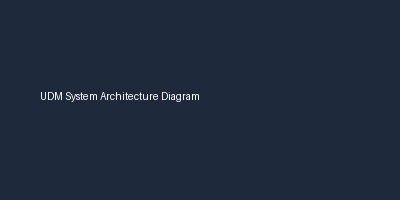
\includegraphics[width=0.8\linewidth]{figures/architecture.png}
\caption{System architecture of the Universal Academic Format Converter.}
\label{fig:arch}
\end{figure}

\section{Conclusion}
We have presented a unified document compiler framework that preserves scientific integrity while ensuring high target template fidelity.

\bibliographystyle{IEEEtran}
\bibliography{references}

\end{document}
